\documentclass[bimj,fleqn]{w-art}
\usepackage{times}
\usepackage{w-thm}
\usepackage[authoryear]{natbib}
\setlength{\bibsep}{2pt}
\setlength{\bibhang}{2em}
\newcommand{\J}{J\"{o}reskog}
\newcommand{\So}{S\"{o}rbom}
\newcommand{\bcx}{{\bf X}}
\newcommand{\bcy}{{\bf Y}}
\newcommand{\bcz}{{\bf Z}}
\newcommand{\bcu}{{\bf U}}
\newcommand{\bcv}{{\bf V}}
\newcommand{\bcw}{{\bf W}}
\newcommand{\bci}{{\bf I}}
\newcommand{\bch}{{\bf H}}
\newcommand{\bcb}{{\bf B}}
\newcommand{\bcr}{{\bf R}}
\newcommand{\bcm}{{\bf M}}
\newcommand{\bcf}{{\bf F}}
\newcommand{\bcg}{{\bf G}}
\newcommand{\bcs}{{\bf S}}
\newcommand{\bca}{{\bf A}}
\newcommand{\bcd}{{\bf D}}
\newcommand{\bcc}{{\bf C}}
\newcommand{\bce}{{\bf E}}
\newcommand{\ba}{{\bf a}}
\newcommand{\bb}{{\bf b}}
\newcommand{\bc}{{\bf c}}
\newcommand{\bd}{{\bf d}}
\newcommand{\bx}{{\bf x}}
\newcommand{\by}{{\bf y}}
\newcommand{\bz}{{\bf z}}
\newcommand{\bu}{{\bf u}}
\newcommand{\bv}{{\bf v}}
\newcommand{\bh}{{\bf h}}
\newcommand{\bl}{{\bf l}}
\newcommand{\be}{{\bf e}}
\newcommand{\br}{{\bf r}}
\newcommand{\bw}{{\bf w}}
\newcommand{\de}{\stackrel{D}{=}}
\newcommand{\bt}{\bigtriangleup}
\newcommand{\bfequiv}{\mbox{\boldmath $\equiv$}}
\newcommand{\bmu}{\mbox{\boldmath $\mu$}}
\newcommand{\bnu}{\mbox{\boldmath $\nu$}}
\newcommand{\bxi}{\mbox{\boldmath $\xi$}}
\newcommand{\btau}{\mbox{\boldmath $\tau$}}
\newcommand{\bgamma}{\mbox{\boldmath $\Gamma$}}
\newcommand{\bphi}{\mbox{\boldmath $\Phi$}}
\newcommand{\bfphi}{\mbox{\boldmath $\varphi$}}
\newcommand{\bfeta}{\mbox{\boldmath $\eta$}}
\newcommand{\bpi}{\mbox{\boldmath $\Pi$}}
\newcommand{\bequiv}{\mbox{\boldmath $\equiv$}}
\newcommand{\bvarepsilon}{\mbox{\boldmath $\varepsilon$}}
\newcommand{\btriangle}{\mbox{\boldmath $\triangle$}}
\newcommand{\bdelta}{\mbox{\boldmath $\Delta$}}
\newcommand{\beps}{\mbox{\boldmath $\epsilon$}}
\newcommand{\btheta}{\mbox{\boldmath $\theta$}}
\newcommand{\balpha}{\mbox{\boldmath $\alpha$}}
\newcommand{\bsphi}{\mbox{\boldmath $\varphi$}}
\newcommand{\bsig}{\mbox{\boldmath $\sigma$}}
\newcommand{\bfpsi}{\mbox{\boldmath $\psi$}}
\newcommand{\bfdelta}{\mbox{\boldmath $\delta$}}
\newcommand{\bsigma}{{\bf \Sigma}}
\newcommand{\bzero}{{\bf 0}}
\newcommand{\bpsi}{\mbox{\boldmath $\Psi$}}
\newcommand{\bep}{\mbox{\boldmath $\epsilon$}}
\newcommand{\bomega}{\mbox{\boldmath $\Omega$}}
\newcommand{\bfomega}{\mbox{\boldmath $\omega$}}
\newcommand{\blambda}{\mbox{\boldmath $\Lambda$}}
\newcommand{\bflambda}{\mbox{\boldmath $\lambda$}}
\newcommand{\bfsigma}{\mbox{\boldmath $\sigma$}}
\newcommand{\bfpi}{{\mbox{\boldmath $\pi$}}}
\newcommand{\bupsilon}{\mbox{\boldmath $\upsilon$}}
\newcommand{\obs}{{\rm obs}}
\newcommand{\mis}{{\rm mis}}
\theoremstyle{plain}
\newtheorem{criterion}{Criterion}
\theoremstyle{definition}
\newtheorem{condition}[theorem]{Condition}
\usepackage[]{graphicx}
\chardef\bslash=`\\ % p. 424, TeXbook
\newcommand{\ntt}{\normalfont\ttfamily}
\newcommand{\cn}[1]{{\protect\ntt\bslash#1}}
\newcommand{\pkg}[1]{{\protect\ntt#1}}
\let\fn\pkg
\let\env\pkg
\let\opt\pkg
\hfuzz1pc % Don't bother to report overfull boxes if overage is < 1pc
\newcommand{\envert}[1]{\left\lvert#1\right\rvert}
\let\abs=\envert


% own packages
\usepackage{siunitx}
\usepackage{enumitem}
\usepackage{placeins} %floatbarrier
% tikz
\usepackage{tikz}
% we want ER + above/below + left/right
\usetikzlibrary{er,arrows, chains, fit, positioning, calc, shapes}

% kableExtra
\usepackage{booktabs}
\usepackage{longtable}
\usepackage{array}
\usepackage{multirow}
\usepackage{wrapfig}
\usepackage{float}
\usepackage{colortbl}
\usepackage{pdflscape}
\usepackage{tabu}
\usepackage{threeparttable}
\usepackage{threeparttablex}
\usepackage[normalem]{ulem}
\usepackage{makecell}
\usepackage{xcolor}

\begin{document}

%\DOIsuffix{bimj.DOIsuffix}
\DOIsuffix{bimj.200100000}
\Volume{52}
\Issue{61}
\Year{2020}
\pagespan{1}{}
\keywords{Adaptive Seamless Designs; Clinical Trials; Model-Based Optimization; Treatment Selection\\\\ %FIXME: name 5 %Up to five keywords are allowed and should be given in alphabetical order. Please capitalize the key
%\noindent \hspace*{-4pc}\\
%\hspace*{-4pc} 
%{\small\it words)}\\[1pc]
\noindent\hspace*{-4.2pc} Supporting Information for this article is available from the author or on the WWW under\break \hspace*{-4pc} \underline{http://dx.doi.org/10.1022/bimj.XXXXXXX} (please delete if not
applicable)
}  %%% semicolon and fullpoint added here for keyword style

\title[Model-based Optimization of Adaptive Seamless Designs]{Optimizing the power of adaptive seamless designs using Bayesian Optimization} %(please use sentence case, e.g. Score tests for exploring complex models)
%% Information for the first author.
\author[Jakob Richter {\it{et al.}}]{Jakob Richter\footnote{Corresponding author: {\sf{e-mail: richter@statistik.tu-dortmund.de}}}\inst{,1}} 
\address[\inst{1}]{Fakultät Statistik, Technische Universität Dortmund, 44221 Dortmund}
%%%%    Information for the second author
\author[dd]{Tim Friede\inst{2}}
\address[\inst{2}]{Institut für Medizinische Statistik, Universitätsmedizin Göttingen, 37073 Göttingen}
%%%%    Information for the third author
\author[]{Jörg Rahnenführer\inst{1}} %please provide full author names. Middle names should be indicated by initials only, i.e. Henry J. James
%%%%    \dedicatory{This is a dedicatory.}
\Receiveddate{zzz} \Reviseddate{zzz} \Accepteddate{zzz} 

\makeatletter
\let\newtitle\@title
\makeatother

% max 250 words
\begin{abstract}
In clinical trials, planning patient group sizes and test methods is a crucial task.
A common goal is to maximize the test power, given a set of treatment and effect sizes under the null hypothesis.
From a wide range of possible alternatives we want to select the best plan in a short period of time, to enable quick decisions.
The standard approach to simulate the power for each single setup can become too time-consuming, when the number of possible setups becomes very large.
Then, either large computational resources are required or an exhaustive exploration of all possible setups takes a very long time.
In this work we propose to use Model-based Optimization to quickly find a clinical trial setup with high power from a large number of setups options.
We demonstrate the effectiveness of our approach by optimizing the power of adaptive seamless designs for different sets of treatment effect sizes.
We compare the MBO approach with an exhaustive evaluation of all candidate designs.
The optimization approach finds competitive setups in a fraction of the time.
\end{abstract}



%% maketitle must follow the abstract.
\maketitle                   % Produces the title.

%% If there is not enough space inside the running head
%% for all authors including the title you may provide
%% the leftmark in one of the following three forms:

%% \renewcommand{\leftmark}
%% {First Author: A Short Title}

%% \renewcommand{\leftmark}
%% {First Author and Second Author: A Short Title}

%% \renewcommand{\leftmark}
%% {First Author et al.: A Short Title}

%% \tableofcontents  % Produces the table of contents.


\section{Introduction}

Clinical research and in particular drug development is typically structured into phases, e.g. phases I to IV in drug development. 
Similar approaches exist for complex interventions, such as the MRC framework for non-pharmacological interventions (ref)%FIXME ref
The development phases include elements of learning and confirmation.
For instance, \citet{sheiner_learning_1997} describe the drug development process as two learning and confirming cycles:
The first cycle includes learning about the tolerated dose (Phase I) and confirming the efficacy of the selected dose in a selected group of patients (Phase IIa), whereas the second cycle consists of learning about the optimal use in representative patients (Phase IIb) and confirming of an acceptable benefit or risk ratio (Phase III).

Traditionally, separate studies are performed for learning and confirming.
However, the landscape in clinical research is changing.
Boundaries between the development phases are increasingly dissolving in multiple aspects.
Master protocols are a new concept where multiple subgroups and substudies are integrated (ref). %FIXME ref
Here, simultaneously, more than one treatment and more than one disease type are investigated within the same overall trial structure.
Adaptive designs are established, but are being further developed.
In general, study designs become more flexible, and more principled approaches to decision making using statistical modeling and integrated analyses across studies become popular. 
A related principle on the analysis side is evidence synthesis, which is a way of combining information from several studies that have examined the same question to come to an overall understanding.

The increasing complexity of both the designs and the analyses of clinical trials has the consequence that the planning of such studies often relies also on computer simulations, especially if no closed form solutions for calculations are available.
This applies even to usually fairly straightforward tasks as sample size calculations. 
Various frameworks and guidance proposals have been developed over the past years on how to plan, execute and interpret the results of such simulation studies.
Method comparison studies are used to give clinicians and biostatisticians guidance when an approach improves currently used methods.  
Depending on the setting and the purpose of the simulation study, suitable metrics must be chosen to compare alternative designs or analysis strategies. 
Especially relevant are neutral comparison studies, which are characterized as follows: %FIXME Is there someting missing? (Jakob)
The primary goal of the respective article is not to introduce a new promising method, the authors are reasonably neutral, and the evaluation metrics, methods, and data sets are chosen in a rational way (ref).
%While method comparison studies aim to make statements when one approach might dominate others in terms of the chosen metrics, in designing an individual study or series of studies the objective is to identify a design that is optimal in terms of the metrics chosen in a certain scenario or, more importantly, across a set of scenarios. 
A comprehensive framework for such an objective assessment of competing strategies for clinical trial designs is CSE (Clinical Scenario Evaluation). ref %FIXME ref
CSE was particularly developed to support the overall process of performing simulations of clinical trials, especially for complex designs and analysis strategies.
The problem is decomposed into data models, analysis models, and evaluation models that specify the evaluation metrics.

Here, we propose to use a formal approach to optimization of the clinical trial design, in the situation of a very large number of available options for the parameters specifying the design. 
This set of candidate designs can be regarded as a multi-dimensional search space, including potentially many real-valued and categorical parameters.
The vast space of possible designs makes the optimization computationally demanding.
In the following, we demonstrate that the so-called Model-based optimization (MBO) framework~\citep{jones_taxonomy_2001} can be successfully applied to select a clinical trial design.
As evaluation metric we consider the specific case that the statistical power of the clinical trial design should be maximized, for given effect sizes and number of treatments.
Further, it is crucial that such a design is found in a short time.
%\subsection{Related work}
%subsub Clinical 
% TODO: Tim

MBO, often also called Bayesian optimization, has been successfully applied to optimize expensive black-boxes in many different scenarios.
Popular applications include hyper-parameter tuning of machine learning methods~\citep{snoek_practical_2012}, general algorithm configuration~\citep{hutter_sequential_2011}, and many more.
Various implementations of MBO methods are used widely, such as SMAC~\citep{hutter_sequential_2011}, Spearmint~\citep{snoek_practical_2012}, and BoTorch~\citep{balandat_botorch_2020}.
For this work we use the implementation in the R-package \texttt{mlrMBO}~\citep{bischl_mlrmbo_2017}.
This implementation has been successfully used to optimize hyper-parameters of machine learning methods on various tasks~\citep{bischl_mlrmbo_2017, wozniak_candle_2018}, and in the biomedical context it has been applied to optimize model-weights~\citep{richter_modelbased_2019,browaeys_nichenet_2020}.
Also, MBO is well suited for multi-criteria optimization.
Different adaptions of MBO exist~\citep{horn_modelbased_2015} that return a set of non-dominated points.
Many of them are implemented in \texttt{mlrMBO} as well.
However, in this work we restrict ourselves to single-criteria optimization. 

The remainder of the manuscript is structured as follows.
In the next section we present as motivating example an application of adaptive seamless designs for chronic obstructive pulmonary disease (COPD).
In the sections~\ref{sec:adaptive_seamless_designs} and~\ref{sec:model_based_optimization}, we explain the background on adaptive seamless designs (asd) and model-based optimization (MBO), respectively.
In section~\ref{sec:simulation_study}, we present a simulation study that is closely related to the motivating example and in which the suitability of MBO for optimizing trial designs is demonstrated.
In the last Section~\ref{sec:discussion}, we discuss promising extensions as well as limitations of the approach.

\section{Motivating Example}
\label{sect.motivation}

The general idea of this paper is to apply MBO for finding a trial design that is optimal with respect to a certain metric.
As an example, we consider the maximization of the statistical power of a trail design, given a set of parameters to be chosen for the trial design.
We compare the computation time as well as the maximal obtained power between the results obtained with MBO and with an exhaustive grid search over the space of adjustable parameters.
The presented optimization approach can also be applied for optimizing other metrics than the power, as long as the metric itself is numeric and the parameters of the trial design are numeric and include none or just few categorical choices.

One specific trial design that falls into this category are \emph{adaptive seamless designs}~\citep{barnes_integrating_2010} as implemented in the \texttt{asd}~\cite{parsons_software_2011} package and described in Section~\ref{sec:adaptive_seamless_designs}.
%(What is THE asd paper? peter bauer, meinter kieser, 1999 statistics in medicine, % https://doi.org/10.1002/(SICI)1097-0258(19990730)18:14%3C1833::AID-SIM221%3E3.0.CO;2-3, ) 
% https://doi.org/10.1002/bimj.200510232
% seamless trials (assoziert)
%  https://doi.org/10.1002/bimj.200510231
In~\citet{friede_adaptive_2020} the authors present an application of \emph{adaptive seamless designs} for chronic obstructive pulmonary disease (COPD).
We will use this COPD study to apply MBO for finding a trial design with maximal statistical power, given the parameters of the respective design options.
%within the given scenarios restrictions.

%phase II III klinische studien je in Phase
% nicht 100% II = stage 1, 
%stage 1 lung function test
%stage 2 

For the COPD trial, an interim treatment selection was performed. 
Indacaterol is a drug administered to COPD patients.
The patients were randomized to four doses of indacaterol (\SI{75}{\micro\gram}, \SI{150}{\micro\gram}, \SI{300}{\micro\gram} and \SI{600}{\micro\gram}), active controls, and placebo control.
As in \citet{friede_adaptive_2020}, here we ignore the active controls.
The primary outcome of the trial was the percentage of days of poor control over 26 weeks of the COPD patients.
Since the recruitment took only a short time, another outcome was required for treatment selection, in this case forced expiratory volume in 1 s (FEV1) at 15 days.
In the original study, the difference in FEV1 compared to placebo at 15 days for the different doses and corresponding confidence intervals were estimated.
From these, standardized effect sizes were estimated as approximately 0.68, 0.82, 0.95, and 0.91 for the four  indacaterol doses \SI{75}{\micro\gram}, \SI{150}{\micro\gram}, \SI{300}{\micro\gram}, and \SI{600}{\micro\gram}, respectively.
For the final outcome days of poor control, also, from real data the standardized effect sizes were estimated.
These were approximately 0.13, 0.17, 0.23, and 0.20, for the four doses.
The approximate sample sizes per arm were 100 patients in stage 1 and 300 patients in stage 2.

In the analysis of \citet{friede_adaptive_2020}, the aim was to select two doses of indacaterol at the interim analysis that are passed to stage 2, resulting in a total sample size $5 \cdot 100 + 3 \cdot 300 = 1,400$ patients. 
In the simulations, a positive correlation between early and final outcomes of 0.4 was assumed.
Further, different settings with continuous early and continuous or binary final outcomes and different treatment selection strategies were compared.


% FIXME Question: 
% What does exactly specifies 'corr'?
% auf der individuen ebene


% TODO: Jakob 
% phase 1 idea something fast
% phase 2
% Describe the study we look at. / The Data
%COPD trial


% What about these three papers?
%\cite{barnes_integrating_2010}
%\cite{donohue_oncedaily_2010}
%\cite{cuffe_when_2014}

% FIXME: Do we really take in this Assurance?
Assurance: \cite{stallard_optimal_2009} in diskussion abhandeln

\section{Adaptive Seamless Designs}
\label{sec:adaptive_seamless_designs}

% TODO: Jakob copy contents from paper
% Is there a condensed version? In Friede et al (2020) it is only explained in detail?
% TODO: Tim
Intro 3- 4 Sätze

\subsection{Two-stage design with treatment selection}
\label{ssec:two_stage_design_with_treatment_selection}

Multi-arm trial; two-stages; treatment selection in interim analysis; final analysis based on combination test approach with closed test principle

% first stage = interrim analysis
% second stage = final analysys
% stick to first second stage througout text but mention interrim here?

\subsection{Selection rules}
\label{ssec:selection_rules}

\paragraph{Epsilion Rule}

\paragraph{Threshold Rule}

\subsection{Clinical scenario evaluation for ASD}
\label{ssec:clinical_scenario_evaluation_for_asd}

\begin{figure}[ht]
\centering
\begin{tikzpicture}[auto,node distance=1cm,align=center,text width = 3cm, inner sep = 0.1cm, font=\sffamily \scriptsize, outer sep= 0cm]
  \node[draw, ellipse, minimum height=1cm, text width=2.5cm] (ClinicalScenarios) at (0,0) {
    \textbf{Clinical scenarios}\\
    Simulation Studies};
  \node[name=block, rectangle split, rectangle split parts=2, draw, above = of ClinicalScenarios] (UnknownPoints)
  { \begin{itemize}[leftmargin=.3cm, topsep=0cm,itemsep=0cm,partopsep=0cm, parsep=0cm]
      \item Treatment effect on early interim outcome.
      \item Treatment effect on late disability outcome
    \end{itemize}
    \nodepart{second} Unknown
  };
  \node[name=block, rectangle split, rectangle split parts=2, draw, anchor = north east] (HistoricalDataPoints) at (UnknownPoints.north west)
  { \begin{itemize}[leftmargin=.3cm, topsep=0cm,itemsep=0cm,partopsep=0cm, parsep=0cm]
      \item Correlation between early interim and late disability outcomes.
    \end{itemize}
    \nodepart{second} Historical data
  };
  %\node[draw, inner xsep=1em, inner ysep=1em, above left = of ClinicalScenarios, fit = (HistoricalDataPoints) (UnknownPoints)] (boxDiseaseSpecific) {};
  \node[draw, text width = 6.2cm, anchor = south west] (DiseaseSpecific) at (HistoricalDataPoints.north west) {\textbf{Disease-specific features}};
  %\node[draw, above right = of ClinicalScenarios] (DesignOptions) {Design options};
  \node[name=block, rectangle split, rectangle split parts=2, draw, anchor = north west] (ConstrainedPoints) at ([xshift = 4cm]HistoricalDataPoints.north east)
  { \begin{itemize}[leftmargin=.3cm, topsep=0cm,itemsep=0cm,partopsep=0cm, parsep=0cm]
      \item Number of test treatments
      \item Total subjects in trial
      \item recruitment rate
    \end{itemize}
    \nodepart{second} Constrained by health care environment/infrastructure
  };
  \node[name=block, rectangle split, rectangle split parts=2, draw, anchor = north west] (CombinationPoints) at (ConstrainedPoints.north east)
  { \begin{itemize}[leftmargin=.3cm, topsep=0cm,itemsep=0cm,partopsep=0cm, parsep=0cm]
      \item Adaptive seamless design time point of interim analysis
      \item Treatment selection rules at interim Conventional phase 2/3
      \item split of resources between phases
      \item end oh phase futility criteria
    \end{itemize}
    \nodepart{second} Combination of options
  };
  \node[draw,text width = 6.2cm, anchor = south west] (DesignOptions) at (ConstrainedPoints.north west) {\textbf{Design Options}};
  \node[draw, below = 0.5cm of ClinicalScenarios] (DesignPerformance) {
    \textbf{Design performance} \\ e.g.\ statistical power};
  \node[draw, right = of DesignPerformance, text width = 4cm, node distance = 2cm] (Evaluation) {
    \textbf{Clinical Scenario Evaluation}\\
    Design performance measures evaluated across a wide range of clinical scenarios};
  \draw[->] (HistoricalDataPoints) -- (ClinicalScenarios);
  \draw[->] (UnknownPoints) -- (ClinicalScenarios);
  \draw[->] (CombinationPoints) -- (ClinicalScenarios);
  \draw[->] (ConstrainedPoints) -- (ClinicalScenarios);
  \draw[->] (ClinicalScenarios) -- (DesignPerformance);
  \draw[->] (DesignPerformance) -- (Evaluation);
\end{tikzpicture}
%FIXME Is this the right paper? Convert to tikz! Tim schickt mir das Original!
%Friede et al (2010) DIJ, Figure 2 https://link.springer.com/content/pdf/10.1177/009286151004400507.pdf? https://link.springer.com/content/pdf/10.1177/009286151004400607.pdf
\caption{Application of the refined clinical scenario evaluation framework to adaptive seamless designs in progressive multiple sclerosis.}
\label{fig:friede_refinement_2010_fig2}
\end{figure}



\subsection{Simulating ASD}
\label{ssec:simulating_asd}
R package asd by Nick Parsons
Test statistics are simulated, not individual participant data

\clearpage

\section{Model-based Optimization}
\label{sec:model_based_optimization}

Sequential \textbf{Model-based Optimization (MBO)}~\citep{jones_taxonomy_2001} (also known as Bayesian optimization) is a state-of-the-art~\citep{shahriari_taking_2016} technique for expensive black-box optimization problems.
In comparison to other black-box optimization methods, like Genetic Algorithms or Simulated Annealing, MBO is especially suitable when evaluating a configuration (e.g.\ running a simulation with certain parameters, here denoted by $\theta$) is very time consuming.
Then it becomes infeasible to evaluate the black-box for thousands of configurations.

\subsection{General principle}
MBO solves an optimization problem within a bounded search space $\Theta$:
\[
\theta^\ast := \operatorname{arg\,max}_{\theta \in \Theta} f(\theta),
\]
where $f(\theta)$ denotes the evaluation of the black-box with the input configuration $\theta$.
To reduce the number of evaluations on $f$ the key idea of MBO is to only evaluate values of $\theta$ that are estimated to lead to a small value of $f(\theta)$.
The estimate is generated by a so called \emph{surrogate model}.
Typically, this is a regression model that predicts the outcome of $f$ based on previous evaluations of $f$.
First, an initial design of already evaluated configurations is needed.
Then, iteratively, the MBO algorithm fits the surrogate on the previous evaluations, proposes a new configuration $\theta$ and evaluates it on $f$.
The steps are repeated until a budget is exhausted.

The proposal of a new configuration $\theta$ is obtained by maximizing a so called acquisition function.
The acquisition function guides the search to promising new regions in the search space $\Theta$ by facilitating the mean prediction $\hat{\mu}(\theta)$ as well as the uncertainty prediction $\hat{s}^2(\theta)$ of the surrogate.
It balances between exploration of not yet evaluated regions in $\Theta$ and exploitation.
The acquisition function achieves exploration by assigning high values to areas where the surrogate predicts a high uncertainty.
Exploitation is achieved by assigning high values to areas of $\theta$ where the surrogate predicts a high outcome of $f$.
For deterministic functions the expected improvement~\citep{jones_efficient_1998} is arguably the most popular acquisition function.

\subsection{Acquisition function for noisy outcomes}
Since this work focuses on optimization of a stochastic simulation, we assume that our non-deterministic optimization problem can be formulated as follows:
\begin{equation}
\theta^\ast := \operatorname{arg\,max}_{\theta \in \Theta} f(\theta) + \varepsilon, \, \text{ with } \, \varepsilon \sim N(0, \sigma^2_{n}) %\text{ i.i.d.}
\end{equation}
In this setting, the expected improvement is not feasible, as shown in \citet{huang_global_2006}.
They propose to use the augmented expected improvement instead.
Therefore, in a first step, we calculate the \emph{effective best solution}:
\begin{equation}
  \theta^{\ast\ast} := \operatorname{arg\,max}\limits_{\theta \in \mathcal{D}} \hat{\mu}(\theta) - c \cdot \hat{s}(\theta),
\end{equation}
with $c$ as a tuning parameter that is usually set to 1 and $\mathcal{D}$ as the design that contains all previously evaluated values of $\theta$.
The effective best point is the pessimistic estimate of the best observed outcome so far.
In the final step, we calculate the augmented expected improvement~\citep{huang_global_2006} as follows:
\begin{multline}
  \label{eq:aei}
  \operatorname{AEI}(\theta) = \left( \hat{\mu}(\theta) - \hat{\mu}(\theta^{\ast\ast}) \right) \cdot  \Phi \biggl( \frac{\hat{\mu}(\theta) - \hat{\mu}(\theta^{\ast\ast})}{\hat{s}(\theta)} \biggr) \\
   + \hat{s}(\theta) \cdot \phi \biggl( \frac{\hat{\mu}(\theta) - \hat{\mu}(\theta^{\ast\ast})}{\hat{s}(\theta)} \biggr) \cdot \biggl(1 - \underbrace{\frac{\sigma_{n}}{\sqrt{\sigma_{n}^2 + \hat{s}^2(\theta)}}}_{\text{correction}}\biggr),
\end{multline}
where $\Phi$ and $\phi$ are the distribution and density function of the standard normal distribution, and $\sigma_{n}^2$ denotes the random error (nugget effect) in the Kriging model.
The formula is derived under the assumption, that at each point $\theta \in \Theta$ the posterior of the function outcome follows a normal distribution.
This assumption is also reflected by using a Gaussian process regression as a surrogate.
The intuition in formula (\ref{eq:aei}) is that the first summand favors exploitation while the second summand favors exploration.
The correction term is necessary to avoid exploration in areas where the model uncertainty $\hat{s}^2(\theta)$ equals the random error $\sigma_{n}^2$, because in this case further evaluations will not decrease the model uncertainty.

\subsection{Selection of the best point from noisy outcomes}
\label{ssec:best_point}
If we chose the configuration $\theta$ from all previously evaluated configurations according to the best outcome of $f$ as the optimization result, we would be overly optimistic.
It is likely that a single best outcome can be partially attributed to the random error $\sigma_{n}^2$.
Instead, we are interested in the optimum of the true posterior mean.
Therefore, we employ the surrogate estimate of the posterior mean for each evaluated configuration to cancel out the noise.
The configuration for which the surrogate estimates the best outcome is then returned as the optimization result $\hat{\theta}^\ast$:
\begin{equation}
  \hat{\theta}^{\ast} := \operatorname{arg\,max}\limits_{\theta \in \mathcal{D}} \hat{\mu}(\theta),
\end{equation}
%To obtain a final outcome $\nu^\ast = f(\theta^\ast)$ that is independent of the optimization process, $f(\theta^\ast)$ is calculated again.
Using the stochastic outcome $\hat{\nu}^\ast := f(\hat{\theta}^\ast) $ observed during the optimization process would still potentially lead to an overly optimistic result.
Therefore an independent calculation of $f(\hat{\theta}^\ast)$ should be conducted to obtain a fair estimate of the true value of the best outcome.

\clearpage

\section{Simulation Study}
\label{sec:simulation_study}

% TODO : Jakob

The goal of this simulation study is to investigate the potential benefit of the MBO approach for effectively finding a clinical trial design that maximizes a metric.
The analysis is motivated by the clinical example with COPD patients introduced in Section~\ref{sect.motivation}, with treatment selection in the first of two stages.
In the first stage five arms (defined by the control and four different administered doses) are considered, and in the second stage only a selected subset of arms is kept for further evaluation. 
The metric to be optimized is the statistical power, where a positive outcome means a trial arm with true effect is detected as significant effect.

\subsection{Clinical trial design and parameters}
\label{subsec:design}
For the true effect sizes in the simulation, we consider four \emph{effect sets} whose values are inspired and partially based on the corresponding numbers of the motivating example, see Table~\ref{tab:table_effect_names}.
\begin{table}

\caption{\label{tab:table_effect_names}Effect sizes used for simulation}
\centering
\begin{tabular}[t]{llrrrrr}
\toprule
\multicolumn{2}{c}{ } & \multicolumn{5}{c}{Treatment} \\
\cmidrule(l{3pt}r{3pt}){3-7}
Effect Set & Stage & 1 & 2 & 3 & 4 & 5\\
\midrule
 & early & 0 & 0.680 & 0.82 & 0.950 & 0.91\\

\multirow{-2}{*}{\raggedright\arraybackslash paper} & final & 0 & 0.130 & 0.17 & 0.230 & 0.20\\
\cmidrule{1-7}
 & early & 0 & 0.200 & 0.40 & 0.600 & 0.80\\

\multirow{-2}{*}{\raggedright\arraybackslash linear} & final & 0 & 0.050 & 0.10 & 0.150 & 0.20\\
\cmidrule{1-7}
 & early & 0 & 0.100 & 0.20 & 0.700 & 0.80\\

\multirow{-2}{*}{\raggedright\arraybackslash sigmoid} & final & 0 & 0.025 & 0.05 & 0.175 & 0.20\\
\cmidrule{1-7}
 & early & 0 & 0.680 & 0.82 & 0.950 & 0.91\\

\multirow{-2}{*}{\raggedright\arraybackslash paper2} & final & 0 & 0.260 & 0.34 & 0.460 & 0.40\\
\bottomrule
\end{tabular}
\end{table}

For the effect set \emph{paper} we use exactly the same numbers as in~\citet{friede_adaptive_2020}.
For the effect set \emph{paper2} the effect sizes for the second stage are doubled.
As further case we consider a \emph{linear} effect set with effect sizes linear increasing from 20\% to 80\% for the first stage and effect sizes divided by 4 for the second stage as well as a \emph{sigmoid} relationship, again with 4 times larger effect sizes for the first stage.
These sets reflect different realistic situations.

The strategies regarding treatment selection for the second stage in the two-phase trial design, following the concept of adaptive seamless designs discussed in Section~\ref{sec:adaptive_seamless_designs}, and their corresponding parameters that are used in the simulation study are given in Table~\ref{tab:selection_strategies} and Table~\ref{tab:search_space}, respectively.
The strategies 1, 2, 3, and \emph{all} select the $k$ best strategies according to their respective test statistics in the first stage (with \emph{all} representing all $k=4$ treatments besides the control). The strategies \emph{eps} and \emph{thresh} represent strategies with a flexible number of treatments taken to the second stage. 
In Table~\ref{tab:search_space} the ranges for these two parameters and for the proportion of patients (ratio $r$) allocated to the second stage are given.
\begin{table}[h]
  \caption{Overview of selection strategies to determine which trial arms are kept for second stage}
  \label{tab:selection_strategies}
  \centering
  \begin{tabular}{ll}
  \hline
  Notation       & Procedure of selection strategy  \\
  \hline
  \emph{all}     & Select all arms  \\
  $\{1,2,3\}$    & Select 1, 2 or 3 arms, respectively, according to maximal test statistic \\
  \emph{eps}     & Select all arms with test statistic less than $\epsilon$ (epsilon) below maximal test statistic \\
  \emph{thresh}  & Select all arms with test statistic larger than the value $\tau$ (threshold) \\
  \hline
  \end{tabular}
\end{table}
\begin{table}[h]
  \caption{Parameters for the selection strategies representing the search space of trial designs}
  \label{tab:search_space}
  \centering
  \begin{tabular}{ll}
  \hline
  Parameter                        & Range \\
  \hline
  Selection strategy               & $\{\text{all}, 1, 2, 3, \text{eps}, \text{thresh} \}$ \\
  $r$ (ratio)                      & $(0,1)$ \\
  $\epsilon$ (only for \emph{eps}) & $[0,4]$ \\
  $\tau$ (onlt for \emph{thresh})  & $[0,10]$ \\
  \hline
  \end{tabular}
\end{table}

%FIXME: JR: uniform naming: eps, thersh for the values and epsilon and treshold for the strategies

\subsection{Calculation of the statistical power}

Let $n_{\text{treat}}$ be the total number of treatments in the overall trial, and let $n_{\text{stage1}}$ and $n_{\text{stage2}}$ be the numbers of patients allocated to each treatment in stage 1 and stage 2 of the trial, respectively. Let $k_1$ and $k_2$ denote the number of treatments in stage 1 and stage 2, respectively. Within one stage, the same number of patients are allocated to all different treatments. Then $n_{\text{treat}}$ is given by
\begin{equation}
  \label{eq:ntreat}
  n_{\text{treat}} = k_1 \cdot n_{\text{stage1}} + k_2 \cdot n_{\text{stage2}}.
\end{equation}
In our scenario (as described in Section \ref{subsec:design}) we have $k_1 = 5$ and $k_2 \in \{2, \ldots, 5\}$, where $k_2$ depends on the result of the treatment selection strategy in stage 1 and the control treatment is included in both stages.

Our main optimization goal is to maximize the statistical power $y$ depending on the trial design. The power can be formulated as a black-box as follows:
\begin{align}
  \label{eq:bbox}
  y & = f(n_{\text{stage1}}, n_{\text{stage2}}, \text{effect set}, \text{selection strategy}, \epsilon, \tau).
\end{align}

The total number of treatments $n_{\text{treat}}$ should be constant in the simulation study, when comparing the efficiency of different designs.
We denote the proportion of patients per treatment in stage 1, compared to patients per treatment in both stages, with 
\begin{align}
  \label{eq:r}
 r & = \frac{n_{\text{stage1}}}{n_{\text{stage1}}+n_{\text{stage2}}}.
\end{align}
Given the number of treatments $k_1$ and $k_2$ in the two stages and the total number of patients $n_{\text{treat}}$, optimizing the power with respect to $n_{\text{stage1}}$ and $n_{\text{stage2}}$ is equivalent to optimizing with respect to $r$, since
\begin{align}
  \label{eq:stagec}
  %\begin{split}
  n_{\text{stage1}} & = 
  n_{\text{stage1}}\cdot \frac{n_{\text{treat}}}{k_1\cdot n_{\text{stage1}}+k_2\cdot n_{\text{stage2}}} = 
  n_{\text{treat}} \cdot \frac{n_{\text{stage1}}}{k_1\cdot n_{\text{stage1}}+k_2\cdot n_{\text{stage2}}} \nonumber \\
  & = n_{\text{treat}}\cdot
  \frac{r}{k_1\cdot
  r+k_2\cdot (1-r)}, \nonumber \\
  n_{\text{stage2}} & =
  n_{\text{treat}}\cdot
  \frac{1-r}{k_1\cdot
  r+k_2\cdot (1-r)}.
  %\end{split}
\end{align}
%For $k_1 = k_2 = 5$, $c$ would be $n_{\text{treat}} \cdot \frac{1}{5}$ because for each arm we can distribute $\frac{1}{5}$ of the treatments across stage 1 and stage 2.
These formulas give the numbers of patients per treatment arm in the two stages, if $k_2$ is known. 
This is only the case for selection strategies 1, 2, and 3.
For the selection strategies \emph{eps} and \emph{thresh}, $k_2$ depends on the outcome of stage 1.
%choice of the \emph{thresh} or \emph{eps} parameter.
In these cases, for given values of $n_{\text{stage1}}$ and $\epsilon$ or $\tau$, respectively, we can  obtain an estimate $\hat{k}_2$ of $k_2$ with a so-called calibration step.
For a set of values for $n_{\text{stage1}}$ in the interval $\left[ \lceil 0.01 \cdot \frac{n_{\text{treat}}}{k_1} \rceil, \lceil \frac{n_{\text{treat}}}{k_1} \rceil \right]$, we simulate stage 1 of the trial multiple times.
We calculate $n_{\text{stage2}} = (1-r)/r\cdot n_{\text{stage1}}$ from formula (\ref{eq:r}) and $\hat{k}_2$ as the average of the resulting values of $k_2$ for all simulations with a fixed value for $n_{\text{stage1}}$.
Then we select the value of $n_{\text{stage1}}$ such that the corresponding number of total patients is closest to $n_{\text{treat}}$.
More precisely, we minimize
\begin{align}
  \label{eq:targettreat}
  \begin{split}
  h(n_{\text{stage1}}) &:= \left( \Big(k_1 \cdot n_{\text{stage1}} + \hat{k}_2 \cdot %\underbrace{
  \frac{1-r}{r} \cdot n_{\text{stage1}}
  %}_{=n_{\text{stage2}}}
  \Big) - n_{\text{treat}} \right)^2
%  \hat{k}_2 &= f(n_{\text{stage1}}, 1, \text{effect set}, \text{Selection strategy}, \text{Epsilon}, \text{Threshold})_{k_2}
  \end{split}
\end{align}
with respect to $n_{\text{stage1}}$, where the estimate $\hat{k}_2$ is obtained as described above dependent on $n_{\text{stage1}}$. 
%$f$ is the simulator black-box from Equation~\ref{eq:bbox}, that gives us the estimated number of $\hat{k}_2$.
%This number is independent of the simulation of the second stage, so we can set $n_{\text{stage2}}$ to 1.
%The value of $\hat{k}_2$ that was observed with the minimal outcome of $h$ is then used to calculate $c$ in equation~\ref{eq:ntreatcc}.

The calibration step is necessary to guarantee that the total number of treatments $n_{\text{treat}}$ is (in average) the same, also for the variable selection strategies $\text{threshold}$ and $\text{epsilon}$. Then the black-box from formula (\ref{eq:bbox}) can be reformulated as 
\begin{equation}
  y = \tilde{f}(n_{\text{treat}}, r, \text{effect set}, \text{selection strategy}, \epsilon, \tau).
\end{equation}
In our simulations, $n_{\text{treat}}$ is considered to be a constant.

Summarizing, in the following we aim to find the clinical design setup, represented by the parameter values for $r$, \emph{effect set}, \emph{Selection strategy}, $\epsilon$ and $\tau$ that yield the highest statistical power, when evaluating $\tilde{f}$.

\subsection{Optimization strategies}

In the simulation study we compare an exhaustive grid search on the parameter space with MBO (Model-based optimization) with respect to both performance (power) and runtime.

First, we describe the \emph{exhaustive grid search} (\emph{Grid}).
For each effect set (see Table~\ref{tab:table_effect_names}) and for each selection strategy, we conduct an exhaustive grid search with a resolution of 25 points per real-valued dimension, i.e.\ one parameter ($r$) for the strategies all, 1, 2, and 3, and two parameters ($r$ and $\epsilon$ or $\tau$, respectively).
This results in a total of $4 \cdot 25 + 2 \cdot 25 \cdot 25 = 1350$ design configurations that are evaluated for each effect set.
Additionally, we will use a subset of this grid of 7 points per dimensions, resulting in $4 \cdot 7 + 2 \cdot 7 \cdot 7 = 126$ design configurations, which we will call \emph{Grid Small}.
Both grids are evaluated with 10 stochastic replications to estimate the variance of the estimated power.

The best point per evaluated grid is determined by selecting the configuration (parameter set) with the best outcome, i.e.\ the largest power.
The corresponding value is generally too optimistic, as the random noise on the estimated value can contribute to the good outcome.
To account for this optimism and report unbiased performance estimates, for each of the 10 replicate simulations, we identify the best configuration and consider the corresponding 9 outcomes of the other 9 replicate simulations, similar to a cross-validation framework in machine learning applications. 
%This eliminates the risk of only reporting outcomes that are optimal by chance.

Next, we describe our realization of the search with the \emph{MBO (Model-based optimization)} approach.
For the application of MBO, we first have to define how the surrogate model that predicts the outcome of $\tilde{f}$ for unknown values of $\theta$ (parameter sets) is generated.
As the regression model for the surrogate we choose Kriging (also called Gaussian process regression) and use the implementation in the R-package \texttt{DiceKriging}~\citep{roustant_dicekriging_2012}, because it is known to work well for fairly low dimensional search spaces.
We configure Kriging to apply the Mattern$\frac{5}{2}$ kernel with an estimated \emph{nugget effect} to account for the noisy response of $f$ and without scaling the input variables to $[0,1]$.

Kriging expects a numerical input, but our search space contains categorical parameters and is even hierarchical.
First, to transform categorical parameters of the search space (see Table~\ref{tab:search_space}) into numerical values we use one-hot encoding.
Furthermore, our search space is hierarchical because the parameters $\epsilon$ and $\tau$ are only active for the respective selection strategies \emph{eps} and \emph{thresh}.
The hierarchical structure introduces inactive values for the configurations ($\theta$), i.e.\ if the \emph{selection strategy} is set to \emph{eps} the parameter $\tau$ of \emph{thresh} is inactive.
If a value is inactive, we set it to a value two times as high as the maximum in its active range (e.g.\ if $\tau$ is inactive it will be set to 20).
This ensures that within the original range the Kriging model is not or only minimally affected by the inactive values.
Note, that this trick only works because we did not scale the input variables to $[0,1]$ and because the estimated covariance of the Mattern$\frac{5}{2}$ kernel is approximately zero for distances greater than $4$.
With the above steps we ensure that the input for the Kriging is purely numeric.

As an acquisition function we choose the $\operatorname{AEI}$ as explained in Section~\ref{sec:model_based_optimization}.
We start MBO with an initial design of $16$ randomly sampled points and allow $100$ further iterations, summing up to a total budget of $116$ evaluated configurations of the simulator $\tilde{f}$.

At the end of the optimization procedure, the best configuration is chosen according to the best prediction obtained on the set of evaluated points as explained in Section~\ref{ssec:best_point}.
Again, overoptimism must be avoided. 
Thus, the best selected configuration (the best parameter set) is then independently evaluated $10$ times again.

The whole MBO procedure is repeated $10$ times to ensure that a single optimization run was not just lucky in finding the optimum.

Additionally we want to investigate whether the results of \emph{MBO} are better then \emph{grid search} because \emph{MBO} can propose configurations within the whole search space and not only limited the grid.
Therefore we introduce \textbf{MBO Grid}.
The optimization is executed as described for \emph{MBO} but with one difference:
At the end we conduct the independent evaluation for the configuration within the \emph{grid} that is closest to the optimal configuration that is proposed by \emph{MBO}.
% Mention that only configurations of the same factor level are looked at?

We expect that \emph{MBO} achieves to find configurations that yield better results than the \emph{grid search} for two reasons.
First, \emph{MBO} will be able to find an optimal configuration that is not restricted to be within the grid but can be between points from the grid.
Second, \emph{MBO} will not choose configurations that were observed to perform well only due to noise.

\subsection{Implementation}

The algorithms used in this study are implemented in R.
For the model-based optimization, the R-package mlrMBO~\citep{bischl_mlrmbo_2017} is used.
For the simulation of clinical trials, the function \texttt{treatsel.sim} of the R-package asd~\citep{parsons_software_2011} is used, with parameter values given in Table~\ref{tab:par_implement}.
\begin{table}[h]
  \caption{Parameter choices for the R function \texttt{treatsel.sim}}
  \label{tab:par_implement}
  \centering
  \begin{tabular}{lll}
  \hline
  Meaning of parameter & Parameter & Value \\
  \hline
  Number of simulation iterations & \texttt{nsim} & $1000$ \\
  Correlation between early and final outcomes & \texttt{corr} & $0.4$ \\
  Test level & \texttt{level} & $0.025$ \\
  Vector of treatment numbers for determining power & \texttt{ptest} & $(3,4)$ \\
  \hline
  \end{tabular}
\end{table}
The vector of treatment numbers for determining power \texttt{ptest} counts rejections of 3 or 4 hypotheses ???.
Note that the parameter \texttt{nsim} denotes the internal simulation iterations of $\tilde{f}$. 
The ten additional stochastic repetitions we conduct for the \emph{grid search} and \emph{MBO} are additional replicates.

% (TODO Not sure what ptest that means)  %jeweils Elementarhypothese 3, 4 verwerfen, gucken wir gar nicht drauf

\subsection{Results}

As explained before, we obtained unbiased results from the exhaustive grid search, the small grid search and the MBO procedure.
Figure~\ref{fig:plot_boxplot_valid_y} shows that \emph{MBO} yields comparable results to the exhaustive \emph{Grid} for each effect set.
\begin{figure}[htb]
\centering
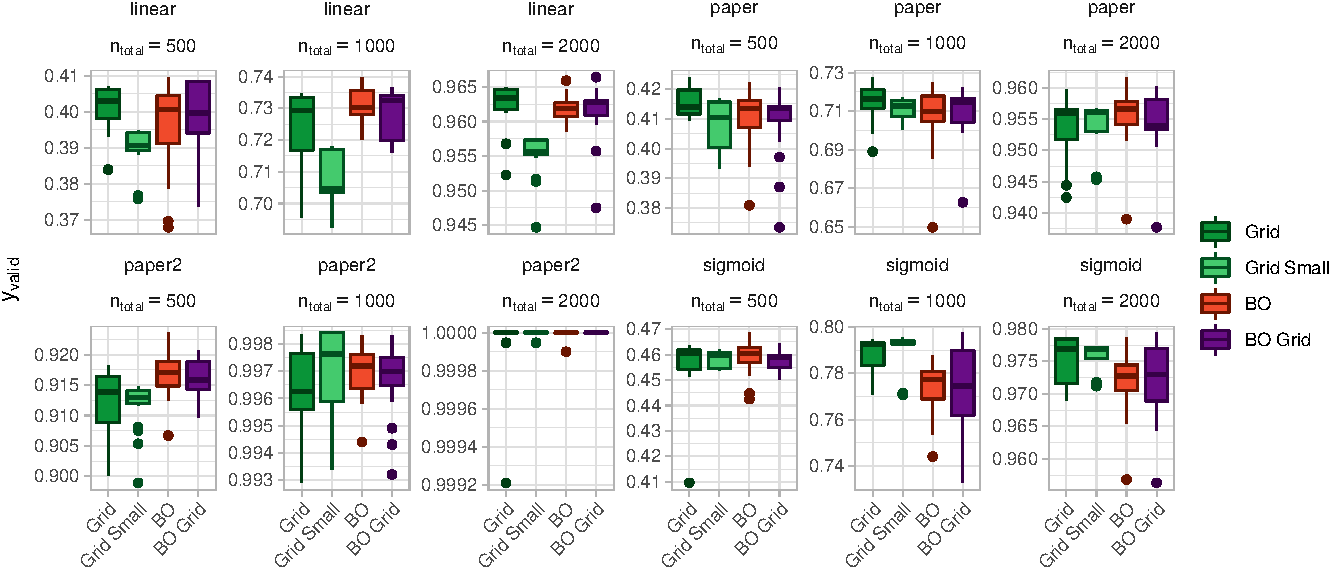
\includegraphics[width=\linewidth]{generated/figures/plot_boxplot_valid_y.pdf}
\caption{%
  Performance on independent replicates of the best found solution from each optimizer for different effect sets and different numbers of $n_{\text{treat}}$. %FIXME rename n_cases in plot
  }
\label{fig:plot_boxplot_valid_y}
\end{figure}
Looking at the results in detail, we can see that in some cases (\emph{effect: linear}, $n_{\text{treat}} = 2000$; \emph{effect: sigmoid}, $n_{\text{treat}} = 1000$; \emph{effect: sigmoid}, $n_{\text{treat}} = 2000$) the exhaustive \emph{Grid} has a slight lead.
In other cases (\emph{effect: linear}, $n_{\text{treat}} = 1000$; \emph{effect: paper2}, $n_{\text{treat}} = 500$; \emph{effect: sigmoid}, $n_{\text{treat}} = 500$) MBO yields slightly better results.
In total \emph{MBO} and the exhaustive \emph{Grid} give equally good results, even though \emph{MBO} is just allowed 116 evaluations in contrast to the 1350 evaluations that are conducted by the \emph{Grid}.
The difference in the number of evaluations is also reflected in the average runtime of each optimization methods given in Table~\ref{tab:table_time}.
\begin{table}

\caption{\label{tab:table_time}Average runtime in hours, for evaluating one grid and one optimization run of MBO.}
\centering
\begin{tabular}[t]{lrrrrrrrrrrrr}
\toprule
\multicolumn{1}{c}{ } & \multicolumn{3}{c}{linear} & \multicolumn{3}{c}{paper} & \multicolumn{3}{c}{paper2} & \multicolumn{3}{c}{sigmoid} \\
\cmidrule(l{3pt}r{3pt}){2-4} \cmidrule(l{3pt}r{3pt}){5-7} \cmidrule(l{3pt}r{3pt}){8-10} \cmidrule(l{3pt}r{3pt}){11-13}
 & 500 & 1000 & 2000 & 500 & 1000 & 2000 & 500 & 1000 & 2000 & 500 & 1000 & 2000\\
\midrule
grid & 55.1 & 60.9 & 60.5 & 62.7 & 63.2 & 204.1 & 59.7 & 64.4 & 67.1 & 54.6 & 52.8 & 61.0\\
mbo & 3.6 & 3.4 & 3.6 & 3.4 & 4.0 & 4.1 & 3.7 & 3.3 & 3.2 & 3.3 & 2.6 & 3.1\\
\bottomrule
\end{tabular}
\end{table}

For the given resolution of 25 points per dimension, the exhaustive \emph{Grid} and the evaluation budget for \emph{MBO}, \emph{MBO} is approximately 20-times faster, while giving equally good results.

Looking at the results of \emph{MBO Grid} in comparison to \emph{MBO} and the exhaustive \emph{Grid}, we can observe two patterns.

First, if \emph{Grid} achieves equal or better results then \emph{MBO}, the results of \emph{MBO Grid} are similar to \emph{MBO}.
In case \emph{MBO} was not able to find a better solution then \emph{Grid}, also \emph{MBO Grid} cannot yield better results as it just takes the configuration on the Grid that is closest to the configuration found by \emph{MBO}.
An increase in performance of \emph{MBO Grid} towards \emph{MBO} could just be by chance.

Second and in contrast to the first pattern: If \emph{MBO} is able to find better configurations then the exhaustive \emph{Grid} (e.g. for scenario \ \emph{effect: linear}, $n_{\text{treat}} = 1000$), also the results of \emph{MBO Grid} are better then the results of \emph{Grid}.
This leads to the conclusion that the resolution of the exhaustive grid is sufficiently fine but the selection of the final configuration within the grid search is faulty in such scenarios.
The grid search has no notion of the stochasticity of the problem.
The configuration that yielded the best outcome is "optimistically" taken as the final configuration.
The independent validation that gives the measure of $y_{\text{valid}}$ shows the unbiased performance of this final configuration. %FIXME: Plot y vs y_valid?
In conclusion we are able to see that even though \emph{Grid} has "seen" all outcomes on the grid, the optimistic choice of the final configuration is indeed overly optimistic and not as good as the final configuration that is determined by the mean prediction of the surrogate of \emph{MBO} as explained in Section~\ref{ssec:best_point}.
In other words, the exhaustive \emph{Grid} is not only extremely demanding in terms of necessary black-box evaluations but also does not take into account the stochasticity of the problem.
We will later study on a single scenario if a reduced noise due to a higher value of \texttt{nsim} decreases the effect of the overly optimistic selection of the \emph{grid search}. %FIXME: n_treat 500, paper 2 would be more interesting or n_treat 1000 and linear)

To compare \emph{MBO} with a grid search that uses approximately the same time  (see~\ref{tab:table_time}) and number of evaluations, we will look at the results of \emph{Grid Small}.
The resolution of 7 points per dimension leads to 126 evaluations which roughly take up the same time as \emph{MBO} (see~\ref{tab:table_time}) with 116 allowed evaluations, giving a small advantage to \emph{Grid Small}.
Despite the 10 more allowed evaluations, in the majority of cases the results of \emph{Grid Small} are inferior the the results of \emph{MBO} as can be seen in Figure~\ref{fig:plot_boxplot_valid_y}.
Only for the scenarios (\emph{effect: paper}, $n_{\text{treat}} = 2000$) and (\emph{effect: sigmoid}, $n_{\text{treat}} = 1000$) \emph{Grid Small} has a small advantage over \emph{MBO} and \emph{Grid}.
For the first scenario the absolute differences are negligible as all methods obtain a high outcome.
For the second scenario we will later see, that the optimal configuration is close to the border of the search space.
The higher resolution of the exhaustive \emph{Grid} probably leads to the selection of slightly suboptimal configurations close to the optimum due to the stochasticity.
These points are not included in the coarse grid.
In other words, if we are lucky and \emph{Grid Small} covers the optimum we are more likely to select it correctly because of less competing candidates.

Note that between the scenarios the absolute differences of the optimization results are of different practical significance, %FIXME "practical significance?"
i.e.\ for scenario (\emph{effect: sigmoid}, $n_{\text{treat}} = 1000$), \emph{Grid} is superior to \emph{MBO} but the difference is smaller than $0.25\%$.

After having looked at the best obtained outcome on our problem scenarios and established the ability of \emph{MBO} to find equally good configurations as the much more demanding exhaustive \emph{Grid} we want to investigate the problems in more detail.
In Figure~\ref{fig:plot_allbest} we show the observed outcomes during evaluation of the grid as well as the final configurations found by MBO, to demonstrate the behavior of the simulation in dependence of the parameters \emph{selection strategy} and \emph{stage ratio} ($r$).
\begin{figure}[htb]
\centering
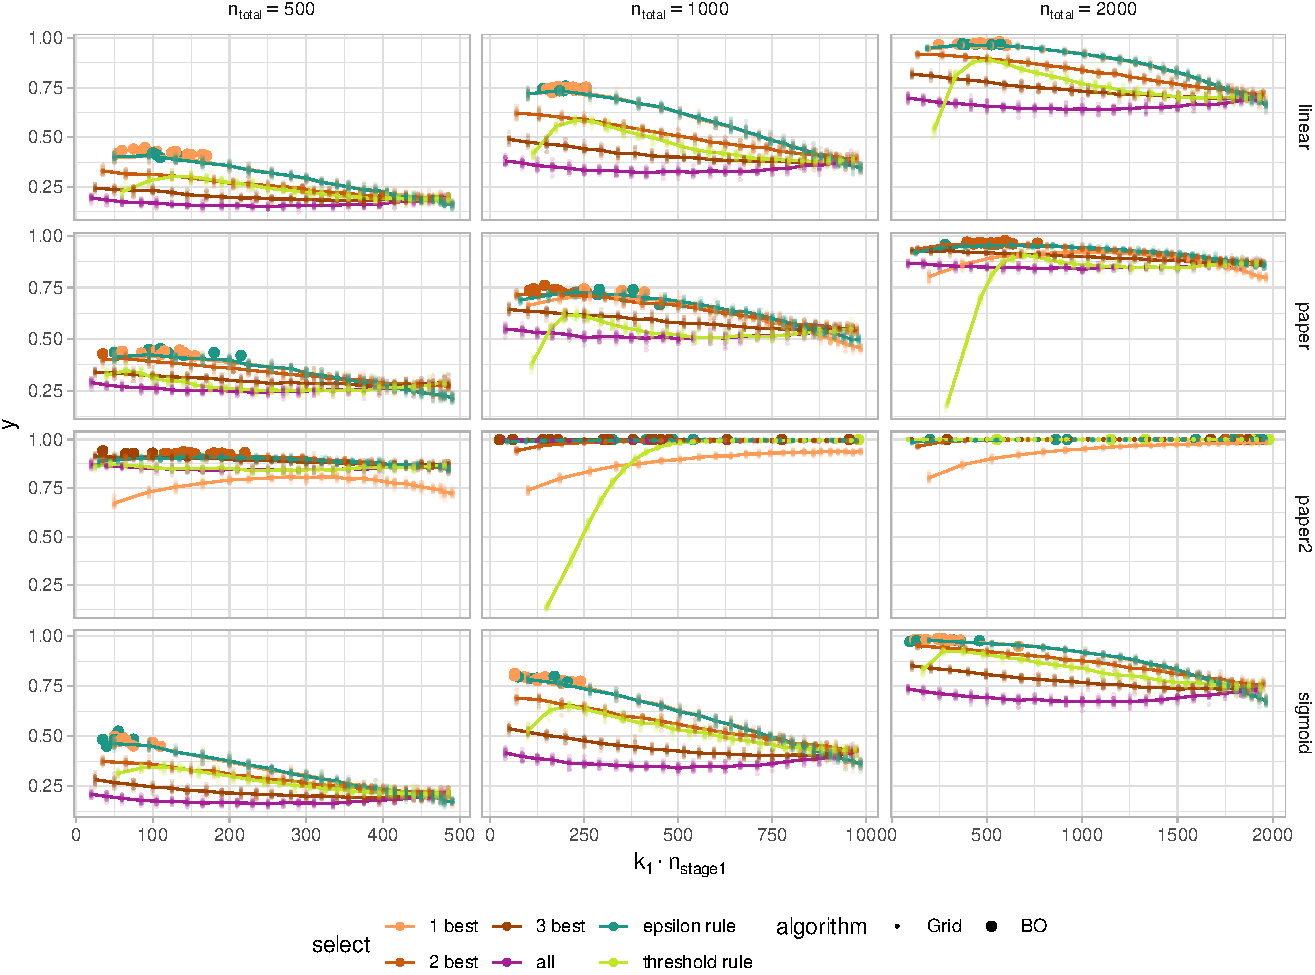
\includegraphics[width=\linewidth]{generated/figures/plot_allbest.pdf}
\caption{%
  All evaluated configurations and their outcomes on the \emph{Grid}.
  For the epsilon and threshold rule only the curve for the $\epsilon$ and $\tau$ value that reached the best power ($y$) is displayed.
  For each configuration in the grid we obtained 10 stochastic results.
  The line connects the mean outcomes for each configuration.
  Additionally the best found configurations from \emph{MBO} are displayed.
  }
\label{fig:plot_allbest}
\end{figure}
Note that the \emph{stage ratio} is not drawn directly but the resulting number of treatments at the first stage.
Also, for the \emph{selection strategy} \emph{epsilon rule} and \emph{threshold rule} only the curves are shown for the $\epsilon$ and $\tau$ value that led to the best outcome within the respective selection strategy.
Also note that for effect set \emph{linear} and \emph{sigmoid} the curves for selection strategy \emph{1 best} and \emph{eps} are nearly identical.
In accordance with intuition, for most scenarios it is the worst decision to use all available treatments in stage 1. 
In all scenarios \emph{MBO} was able to identify the peak of all curves in combination.
Within the 10 stochastic repetitions \emph{MBO} found different configurations that all yield similarly good outcomes.
That no unique best setting was found across the repetitions can be attributed to the relatively high noise of the simulation and the relatively flat peaks, i.e. different configurations yield similarly good outcomes.
In case multiple optimization runs give different configurations it might be advisable to let a human expert choose the final configuration.
%FIXME: Write more about the meaning of the results from a clinical point of view.

In contrast to Figure~\ref{fig:plot_allbest}, Figure~\ref{fig:plot_best_x} shows the outcome of the independent validation and the ratio $r$ directly.
\begin{figure}[htb]
\centering
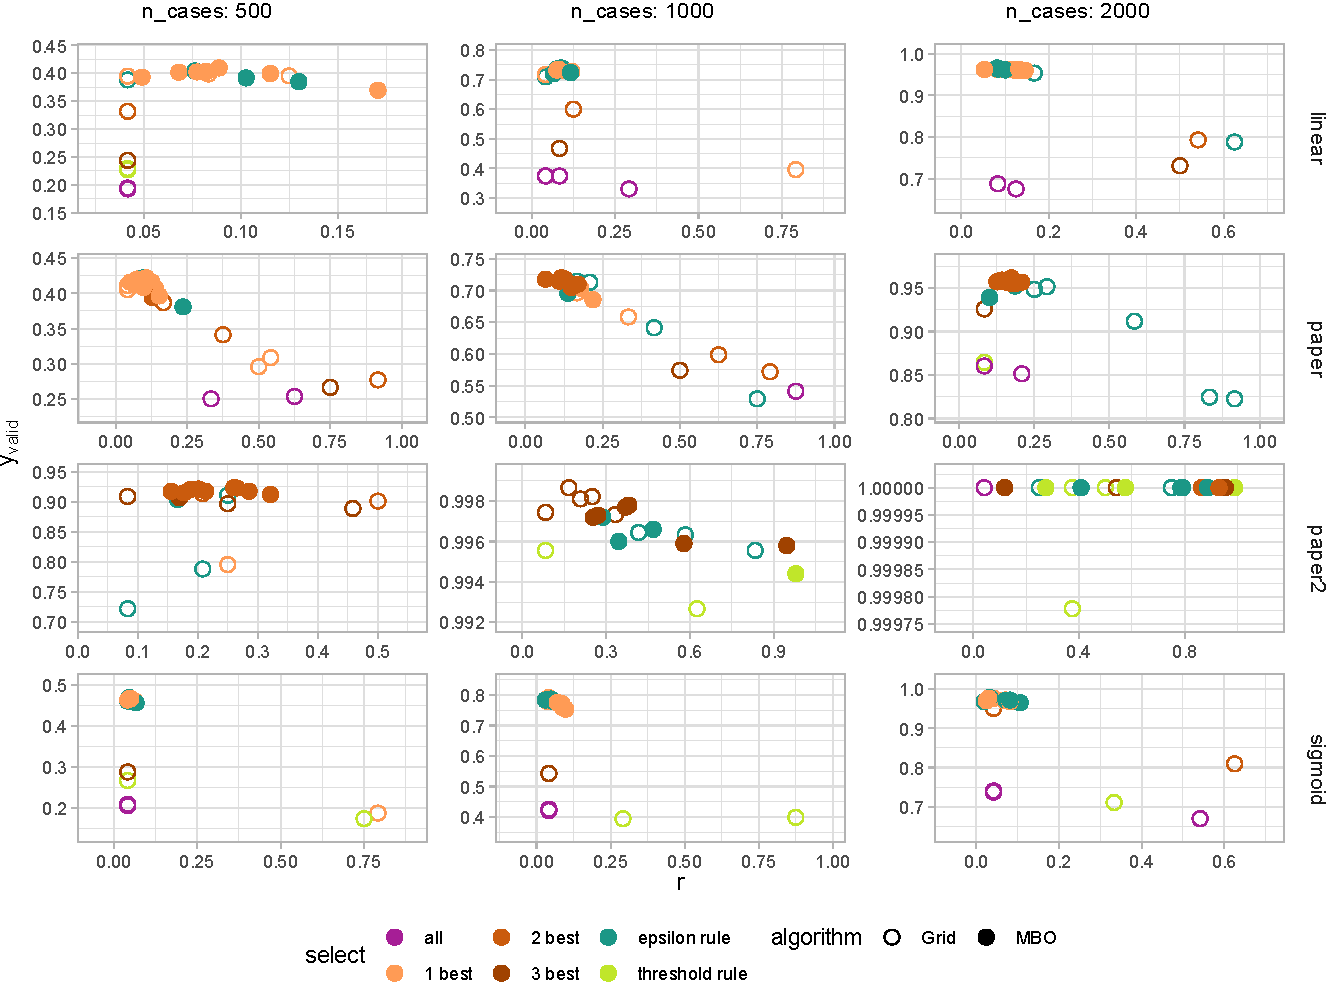
\includegraphics[width=\linewidth]{generated/figures/plot_best_x.pdf}
\caption{Best found $x$-values from MBO runs.}
\label{fig:plot_best_x}
\end{figure}
The results show that for some scenarios most replications of the \emph{Grid} returned the same optimal configurations (e.g.\ for scenario \emph{effect: sigmoid}, $n_{\text{treat}} = 1000$)
In such cases the signal to noise ratio was high enough to reliably find the best configuration.
These are also the scenarios where \emph{Grid} was superior the \emph{MBO} as can be seen in the previously shown Box plots in Figure~\ref{fig:plot_boxplot_valid_y}.
In other cases \emph{Grid} found varying configurations and \emph{MBO} found more stable results that lead to better outcomes (e.g.\ \emph{effect: linear}, $n_{\text{treat}} = 1000$; \emph{effect: paper2}, $n_{\text{treat}} = 500$; \emph{effect: sigmoid}, $n_{\text{treat}} = 500$).
A special scenario is \emph{effect: paper2}, $n_{\text{treat}} = 2000$: Here nearly all found configurations yield perfect outcomes.

\subsection{More simulation rounds}

%FIXME TODO by Jakob

To investigate the effect of the function noise variance ($\sigma^2_n$) on the optimization result we increased the simulation iterations from $n_\text{sim} = 1000$ to $n_\text{sim} = 5000$ for the scenario with the \emph{paper} effect set and  $n_{\text{treat}} = 2000$.
This is expected to increase the runtime by a factor of 5.
Also we expect that due to the decreased noise variance the grid search might be less prone to select over optimistic configurations.
Furthermore, MBO might need less iterations because the signal to noise ratio is higher.

Figure~\ref{fig:plot_opt_path_5000} shows that the lower noise level leads to more stable simulation runs, meaning that a single optimization run leads to a results closer to the mean result.
Also the outcome of the best found point by MBO is closer to the best outcome found by the exhaustive grid search.
We have to remember that this plot reports the best observed outcome so far. 
However, as explained in Section~\ref{ssec:best_point} the best point is not determined by the best found outcome but by the surrogates mean prediction of all evaluated point.
This "bias correction" seems to be effective, as the validation error reported in Figure~\ref{fig:plot_boxplot_valid_y_5000} is nearly identical for MBO in both cases.
Interestingly the validation error of the grid search is lower for $n_\text{sim} = 5000$ then for $n_\text{sim} = 1000$.
We would have expected the opposite, since more noise during optimization leads to overly optimistic choices that result in a bad validation error.
This does not seem to be the case here but also the results are not drastically different and the illustrated IQR for the grid search becomes smaller for $n_\text{sim} = 5000$.

%FIXME: Add Runtime comparision!

\begin{figure}[htb]
\centering
  \begin{minipage}{0.62\textwidth}
    \centering
    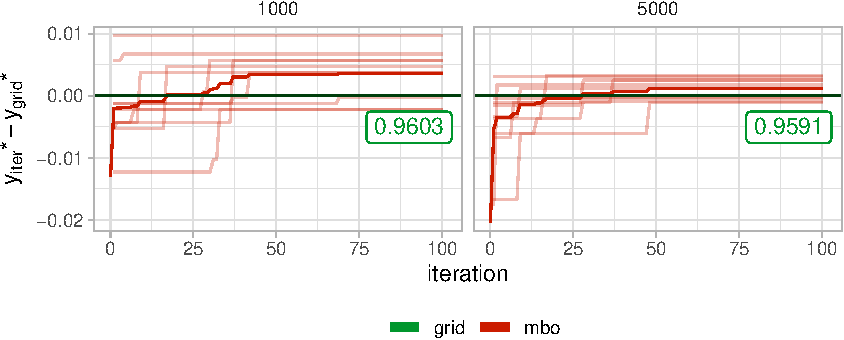
\includegraphics[width=\linewidth]{generated/figures/plot_opt_path_5000.pdf}%
    \captionof{figure}{Optimization progress for \emph{MBO} in each stochastic repetition in comparison to the best found outcome in the grid search on effect set \emph{paper} and $n_{\text{treat}} = 2000$.}
    \label{fig:plot_opt_path_5000}
  \end{minipage}\hspace{0.02\textwidth}%
  \begin{minipage}{0.35\textwidth}
    \centering
    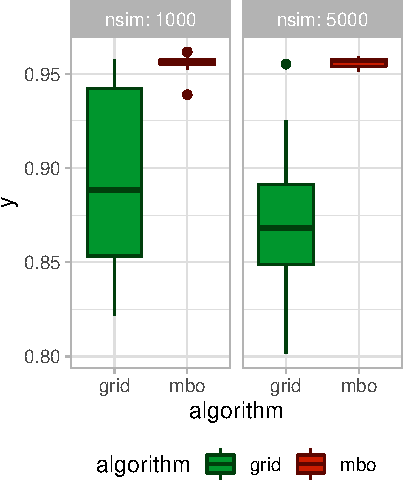
\includegraphics[width=\linewidth]{generated/figures/plot_boxplot_valid_y_5000.pdf}%
    \captionof{figure}{Validated performance of all optimization strategies on effect set \emph{paper} and $n_{\text{treat}} = 2000$ with 100 stochastic repetitions and different values for \texttt{nsim}}
    \label{fig:plot_boxplot_valid_y_5000}
  \end{minipage}
\end{figure}


% This is the body text. Please note that cross-references in the body text should be shown as follows:
% (Miller, 1900), (Miller and Baker, 1900) or if three or more authors (Miller {\it{et al}}., 1900)
% \vspace*{12pt}

% \noindent Bullet lists are not allowed. Always use (i), (ii), etc.
% \vspace*{12pt}

% \noindent Sentences should never start with a symbol.
% \vspace*{12pt}

% \noindent Names of software packages and website addresses should be written in {\texttt{Courier new, i.e. Stata, the R package
% MASS, http://www.biometrical-journal.com.}}

\section{Discussion}
\label{sec:discussion}

% subsection Summary

% subsection Outlook

Instead of keeping the number of total trials constant, we could apply multi-criteria optimization and include this number as an additional outcome.
This multi-criteria approach would result in a set of points (Pareto front) that minimize the number of trails as well as maximize the statistical power of the trail design.
The user could then see for which number of trails the power is above a certain threshold (e.g. $95\%$).

Another way of speeding up the optimization would be to adaptively increase the iterations of the design simulation. 
If few simulations already indicate a bad outcome it might not be promising to evaluate more simulation runs.
Such procedure can be guided through statistical testing and is already common in machine learning under the terms racing or multi-fidelity optimization.

% \begin{table}[htb]
% \begin{center}
% \caption{The caption of a table.}
% \begin{tabular}{lll}
% \hline
% Description 1 & Description 2 & Description 3\\
% \hline
% Row 1, Col 1 & Row 1, Col 2 & Row 1, Col 3\\
% Row 2, Col 1 & Row 2, Col 2 & Row 2, Col 3\\
% \hline
% \end{tabular}
% \end{center}
% \end{table}
% \begin{equation}
% \left({\theta^{0}_{i}}\atop{\theta^{1}_{i}}\right) \sim N(\theta,\Sigma),\quad {\mathrm{with}}\ 
% {{\theta}} = \left({\theta_{0}}\atop{\theta_{1}}\right)\ {\mathrm{and}}\ \Sigma =
% \left(\begin{array}{cc}
% \sigma^{2}_{0} & \rho\sigma_{0}\sigma_{1}\\
% \rho\sigma_{0}\sigma_{2} & \sigma^{2}_{1}
% \end{array}\right).
% \end{equation}

\noindent This is the body text. Only number equations which are referred to in the text body. If equations
are numbered, these should be numbered continuously throughout the text. Not section wise! Please
carefully follow the rules for mathematical expressions in the ``Instructions to Authors''.

\begin{acknowledgement}
This work was partly supported by Deutsche Forschungsgemeinschaft (DFG) within the Collaborative Research Center SFB 876, A3.
\end{acknowledgement}
\vspace*{1pc}

\noindent {\bf{Conflict of Interest}}

\noindent {\it{The authors have declared no conflict of interest.}} %(or please state any conflicts of interest)

%\section*{Appendix {\it(please insert here, if applicable)}}

%\subsection*{A.1.\enspace Second level heading}

%Please insert appendices before the references.


\bibliographystyle{biometrical}
\bibliography{literature,literature_zotero}

\newpage
\phantom{aaaa}
%%%%%%%%%% Merge with supplemental materials %%%%%%%%%%
\clearpage
\begin{center}
\textbf{\large Supplemental Materials: \newtitle}
\end{center}
\FloatBarrier
%%%%%%%%%% Merge with supplemental materials %%%%%%%%%%
%%%%%%%%%% Prefix a "S" to all equations, figures, tables and reset the counter %%%%%%%%%%
\setcounter{equation}{0}
\setcounter{figure}{0}
\setcounter{table}{0}
\setcounter{page}{1}
\makeatletter
\renewcommand{\theequation}{S\arabic{equation}}
\renewcommand{\thefigure}{S\arabic{figure}}
\renewcommand{\thetable}{S\arabic{table}}
\renewcommand{\bibnumfmt}[1]{[S#1]}
%%%%%%%%%% Prefix a "S" to all equations, figures, tables and reset the counter %%%%%%%%%%

\begin{table}

\caption{Best configurations per ncases and effects}
\centering
\fontsize{6}{8}\selectfont
\begin{tabular}[t]{lrlrrr}
\toprule
effect & n\_cases & select & stage\_ratio & epsilon & mean\_y\\
\midrule
 &  & epsilon rule & 0.042 & 0.000 & 0.401\\

 &  & 1 best & 0.083 &  & 0.405\\

 &  & epsilon rule & 0.083 & 0.000 & 0.407\\

 & \multirow{-4}{*}{\raggedleft\arraybackslash 500} & mbo &  &  & 0.422\\
\cmidrule{2-6}
 &  & epsilon rule & 0.083 & 0.167 & 0.729\\

 &  & 1 best & 0.083 &  & 0.731\\

 &  & epsilon rule & 0.083 & 0.000 & 0.735\\

 & \multirow{-4}{*}{\raggedleft\arraybackslash 1000} & mbo &  &  & 0.744\\
\cmidrule{2-6}
 &  & epsilon rule & 0.083 & 0.000 & 0.965\\

 &  & epsilon rule & 0.083 & 0.333 & 0.965\\

 &  & epsilon rule & 0.083 & 0.167 & 0.965\\

\multirow{-12}{*}{\raggedright\arraybackslash linear} & \multirow{-4}{*}{\raggedleft\arraybackslash 2000} & mbo &  &  & 0.970\\
\cmidrule{1-6}
 &  & 1 best & 0.125 &  & 0.417\\

 &  & epsilon rule & 0.083 & 0.167 & 0.421\\

 &  & epsilon rule & 0.083 & 0.000 & 0.424\\

 & \multirow{-4}{*}{\raggedleft\arraybackslash 500} & mbo &  &  & 0.435\\
\cmidrule{2-6}
 &  & epsilon rule & 0.167 & 0.500 & 0.719\\

 &  & epsilon rule & 0.125 & 0.500 & 0.723\\

 &  & epsilon rule & 0.125 & 0.333 & 0.728\\

 & \multirow{-4}{*}{\raggedleft\arraybackslash 1000} & mbo &  &  & 0.731\\
\cmidrule{2-6}
 &  & 2 best & 0.167 &  & 0.956\\

 &  & 2 best & 0.208 &  & 0.957\\

 &  & 2 best & 0.125 &  & 0.960\\

\multirow{-12}{*}{\raggedright\arraybackslash paper} & \multirow{-4}{*}{\raggedleft\arraybackslash 2000} & mbo &  &  & 0.965\\
\cmidrule{1-6}
 &  & 2 best & 0.208 &  & 0.915\\

 &  & 2 best & 0.292 &  & 0.917\\

 &  & 2 best & 0.250 &  & 0.919\\

 & \multirow{-4}{*}{\raggedleft\arraybackslash 500} & mbo &  &  & 0.929\\
\cmidrule{2-6}
 &  & 3 best & 0.250 &  & 0.998\\

 &  & 3 best & 0.208 &  & 0.998\\

 &  & 3 best & 0.167 &  & 0.998\\

 & \multirow{-4}{*}{\raggedleft\arraybackslash 1000} & mbo &  &  & 1.000\\
\cmidrule{2-6}
 &  & all & 0.042 &  & 1.000\\

 &  & 3 best & 0.042 &  & 1.000\\

 &  & all & 0.083 &  & 1.000\\

\multirow{-12}{*}{\raggedright\arraybackslash paper2} & \multirow{-4}{*}{\raggedleft\arraybackslash 2000} & mbo &  &  & 1.000\\
\cmidrule{1-6}
 &  & epsilon rule & 0.042 & 0.167 & 0.455\\

 &  & 1 best & 0.042 &  & 0.462\\

 &  & epsilon rule & 0.042 & 0.000 & 0.463\\

 & \multirow{-4}{*}{\raggedleft\arraybackslash 500} & mbo &  &  & 0.479\\
\cmidrule{2-6}
 &  & epsilon rule & 0.042 & 0.167 & 0.772\\

 &  & epsilon rule & 0.042 & 0.000 & 0.784\\

 &  & mbo &  &  & 0.787\\

 & \multirow{-4}{*}{\raggedleft\arraybackslash 1000} & 1 best & 0.042 &  & 0.794\\
\cmidrule{2-6}
 &  & epsilon rule & 0.042 & 0.167 & 0.972\\

 &  & 1 best & 0.042 &  & 0.977\\

 &  & mbo &  &  & 0.978\\

\multirow{-12}{*}{\raggedright\arraybackslash sigmoid} & \multirow{-4}{*}{\raggedleft\arraybackslash 2000} & epsilon rule & 0.042 & 0.000 & 0.979\\
\bottomrule
\end{tabular}
\end{table}


\begin{figure}[htb]
\centering
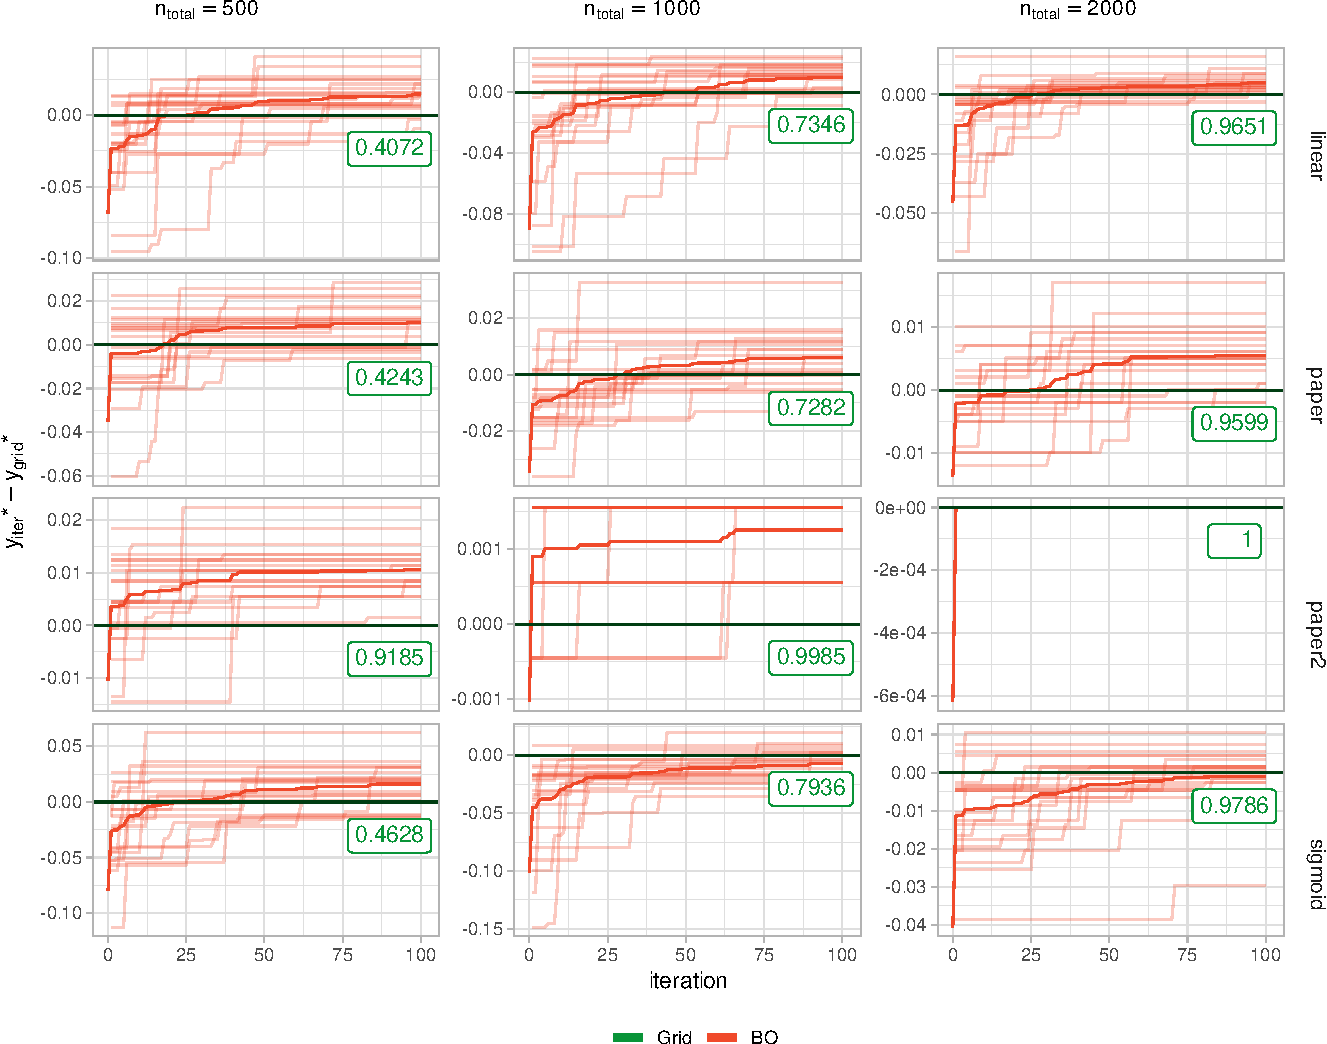
\includegraphics[width=\linewidth]{generated/figures/plot_opt_path.pdf}
\caption{%
  Optimization curves of each optimization run and the mean of all runs drawn as a black line.
  }
\label{fig:plot_opt_path} 
\end{figure}

\end{document}
